%
We will here investigate how our results scales with $B$.
The comparison of the profiles in the steady state will be given together with the results from the saturated turbulent phase.
The comparison of the linear phase is already given in \cref{chap:linear}.

Notice that only $B_0 = 0.06\T \to 0.1\T$ reaches the steady state as $B_0 = 0.02$ is stable against the perturbation and $B_0 = 0.04$ has a very slow growth rate.

Notice that $B_0$ does not appear directly in the normalized equations.
By looking at \cref{eq:celma_vortD,eq:celma_dens,eq:celma_mom_dens,eq:celma_j_par,eq:celma_vortD_evolution}, we can see that that the normalization $B$ can always be chosen to be $1$.
However, $B$ appears in the set of equations through $\om_{ci}$, which means that it effectively sets the time step (in real variables) through $\breve{t}=t\om_{ci}^{-1}$.
This in turn affects the $\rho_s$ (as $\rho_s=\frac{c_s}{\om_{ci}}$), and thus the normalized domain size.

\section{The steady state profiles}
%
\Cref{fig:linBScanPar} shows the parallel profile variations as a function of $B_0$.
%
\begin{figure}[htb]
    \centering
    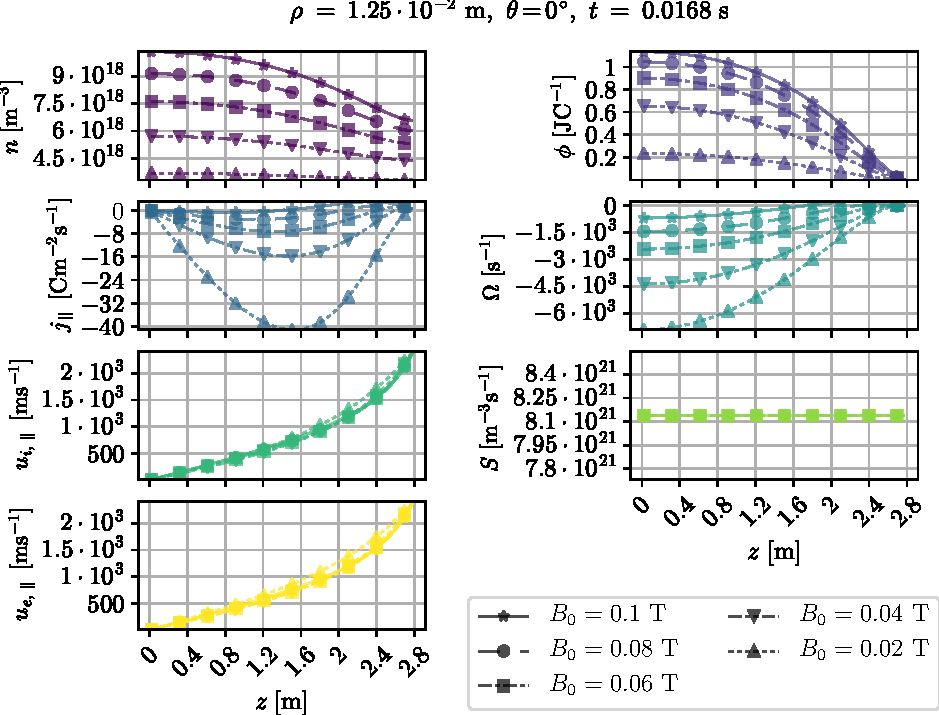
\includegraphics{fig/results/bScan/BScanPar}
    \caption{The parallel steady state profiles as a function of $B_0$.}
    \label{fig:linBScanPar}
\end{figure}
%
We note that $n$ is increasing with increasing $B$-field.
This can be explained by the increase in parallel velocities, which will be further explained in the discussion of the radial profiles.
Although $j_\| \propto n$, we can observe that the absolute magnitude decreases with increasing $B$, signifying that the parallel electron and ion velocities are closer to each other.
As a consequence, the parallel derivatives of $j_\|$ decreases, which in turn means that the absolute amplitude of the vorticity decreases.
$\phi$ retains a Boltzmann-like distribution for all $B$-fields, which means that $\phi$ must decrease in the parallel direction as $n$ decreases.

%
\begin{figure}[htb]
    \centering
    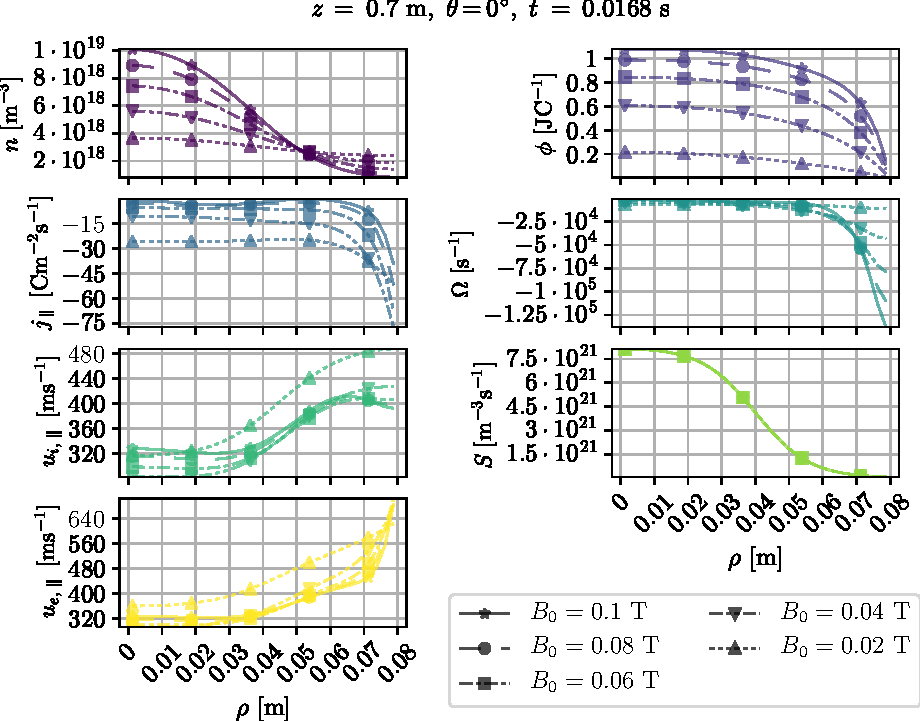
\includegraphics{fig/results/bScan/BScanRad}
    \caption{The radial steady state profiles as a function of $B_0$.}
    \label{fig:linBScanRad}
\end{figure}
%
As indicated in the radial direction in \cref{fig:linBScanRad}, $\phi$ is increasing with increasing $B$-field due to the Boltzmann-like distribution for each parallel position.
Since the potential is fixed to $0$ at $\rho = L_\rho$, we must have that the gradients gets sharper for increasing $B$-fields.
This has the consequence that the vorticity gets higher for increasing $B$.

From this, we will give an explanation for the observed increase in $n$ for increasing $B$ here.
As mentioned in \cref{sec:fluxes}, almost no plasma can leave the domain in the perpendicular direction due to the boundary condition $\L.\phi\R|_{L_\rho}=0$ and shallow parallel second derivatives.
Hence, we must mechanisms in which the plasma can leave the domain in the parallel direction.
We note that the in the parallel momentum equation, the right hand sides equals to first order $-T_i \grad_\| n + q_\a \grad_\| \phi$.
As the parallel gradients increases for increasing $B$ field, the pressure cannot account for the increased parallel outflux.
On the other hand, the potential term can account for at least part of the increased parallel outflux.
As the sign of this term depends on the species types, there will be less difference in this term for lower values of $B$, and since the system seeks a steady state the ions will slow the electron flux less.
However, as the decrease in $\grad_\| \phi$ comes from the decrease in $n$ with decreasing $B$, it cannot account for the initial depletion of density for decreasing $B$.
Is it possible that this initial depletion can come from the fact that the systems searches for balance between the parallel currents and $\Omega$ in order to reach the steady state.

Finally, it is worth nothing that the artificial viscosity is kept constant in the normalized eqautions.
This means that they will increase for decreasing $B$, as they are normalized with $\om_{ci}$.
However, they are small compared with the other terms, and can therefore not account for the trend in $n$ when the magnetic field strength changes.

\section{Variations in turbulence}
%
Evidently less turbulent amplitude
All cases flattening of profiles, but less intensity of the turbulence as shown in \cref{fig:BScanPosOfFluct}
%
\begin{figure}[htb]
    \centering
    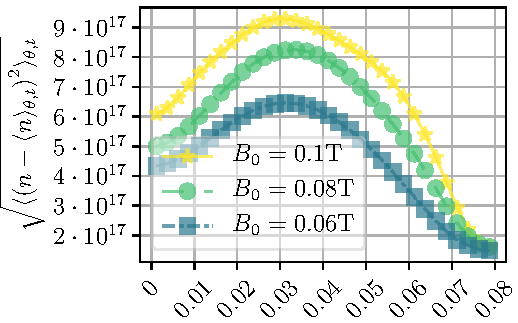
\includegraphics{fig/results/bScan/BScanPosOfFluct}
    \caption{The standard deviation for the turbulent cases.}
    \label{fig:BScanPosOfFluct}
\end{figure}
%
Skew kurt in \cref{fig:BScanSkewKurt}
%
\begin{figure}[htb]
    \centering
    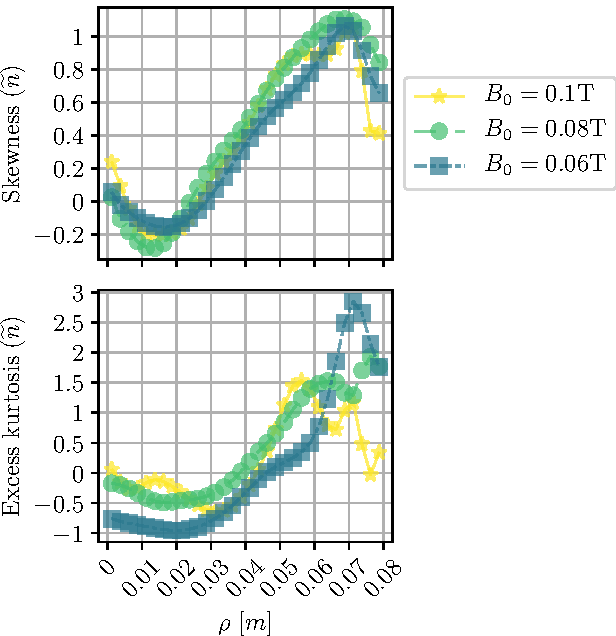
\includegraphics{fig/results/bScan/BScanSkewKurt}
    \caption{The skewness and kurtosis for the turbulent cases.}
    \label{fig:BScanSkewKurt}
\end{figure}
%
Turbulent flux goes down as indicated in \cref{fig:BScanTotalFlux}
%
\begin{figure}[htb]
    \centering
    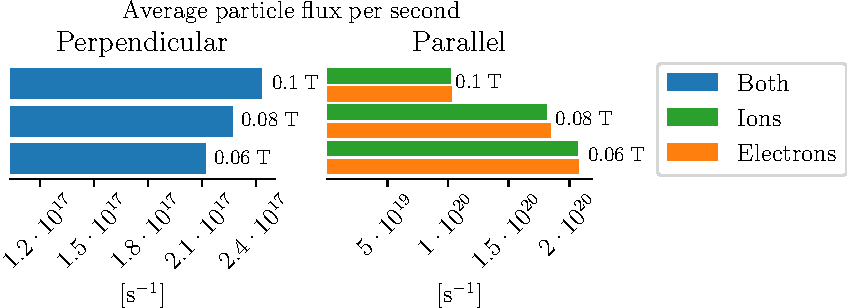
\includegraphics{fig/results/bScan/BScanTotalFlux}
    \caption{The variation of the total flux as a function of $B_0$.}
    \label{fig:BScanTotalFlux}
\end{figure}
%
Less blob as depicted in \cref{fig:BScanBlobCount}
%
\begin{figure}[htb]
    \centering
    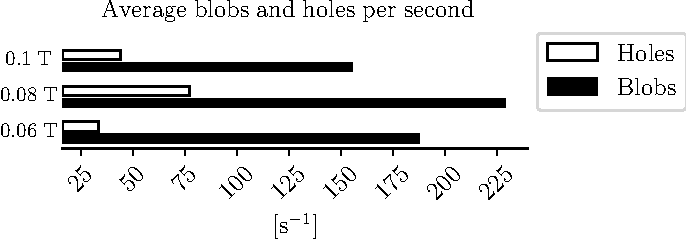
\includegraphics{fig/results/bScan/BScanBlobCount}
    \caption{The blob count as a function of $B_0$.}
    \label{fig:BScanBlobCount}
\end{figure}
%
